
% Defining the chapter
\chapter{Problem Formulation}

In this chapter, the research problem of this dissertation is determined as the problem of combining modern WebTransport over QUIC protocol \cite{rfc9000} with Kubernetes \cite{kubernetes-docs}. WebTransport \cite{webtransport-draft}, QUIC, Kubernetes are very sophisticated technologies, and integrating the 3 technologies to provide real-time and low latency applications is challenging. This chapter addresses the research gaps based on the State of the Art with additional aspects of it and proposes a new solution to these problems and a clear plan to solve. It also discusses the difference between the proposed methodology and the current methods and provides certain design and implementation objectives in order to obtain a sustainable, production-ready streaming framework.

This chapter effectively explains the problem it wants to address, offers an abstracted solution, tells how the work is different among other solutions and provides a blueprint on how the designed solutions could be attained.

% Section 3.1: Identified Challenges
\section{Identified Challenges}
The State of the Art review highlights that there is substantial advancement in modern transport protocols, cloud-based networking as well as streaming platforms. But it also highlights the issues that act against formation of high-performance and real-time systems in kubernetes. The need to conduct this research is motivated by the following challenges, some of which are briefly explained below.

\subsection{Limited Support for QUIC and HTTP/3 in Kubernetes Ingress Controllers}
Experimental QUIC and HTTP/3 support have been added to Kubernetes Ingress Controllers such as NGINX \cite{nginx-ingress-docs}, HAProxy \cite{haproxy-docs}, and Envoy \cite{envoy-proxy} via controller specific annotations such as \texttt{nginx.org/quic: "true"}. Nevertheless, such implementations are unreliable and not production ready. Nginx Controller currently does not support proxying and HAProxy fails to proxy streams. The Gateway Application Programming Interface (API) \cite{gateway-api} has a more open model, and allows protocols that use UDP such as QUIC, and its utility relies on the capabilities of underlying reverse proxies.

Moreover, proxies like Angie \cite{angie-docs} and HAProxy \cite{haproxy-docs} along with the ingress controller cannot inspect or manage individual QUIC streams. This limitation prevents features like stream-aware routing, prioritization, etc which are essential for low-latency applications such as real-time streaming or telemetry. As a result, building efficient, stream-aware systems in Kubernetes remains a challenge.

\subsection{Challenges in Load Balancing for QUIC-Based Traffic}
Unlike the traditional TCP-based protocols, QUIC uses UDP, so it becomes a challenge in Kubernetes environments where the traffic is heavily built on TCP traffic. The cloud service providers, such as Google Cloud, has already implemented support of QUIC in their load balancers with protocol downgrade, whereas on-premise load balancer implementations, such as MetalLB \cite{metallb-docs}, do not have advanced features such as supporting stream-level routing, autoscaling, or failover. MetalLB doesn't support QUIC proxying and treats HTTP as UDP packets. This creates a challenge in managing QUIC-based traffic in a cluster, which is on-prem, local or privately owned, thus encapsulating the scalability of HTTP/3 applications.


\subsection{Operational Complexity and Observability}

QUIC’s encrypted headers and multiplexed streams in QUIC improve performance and security at the expense of making traffic inspection difficult. Kubernetes environment being largely based on tcp have weak weak support for QUIC, which makes it harder to debug and analyze performance as discussed in Section 2.6.10.6. Even the Gateway API decouples infrastructure and application considerations, a misconfiguration of work makes whole operation within kubernetes more difficult as also covered in Section 2.6.10.6. These issues create barriers to building reliable, real-time webtransport stream demultiplexers/Routers in kubernetes.

% Section 3.2: Abstracted View of the Solution
\section{Abstracted Solution}


The aim of this dissertation is to open a possibility of allowing independent WebTransport streams to be load balanced to various microservices that run on Kubernetes and  address the critical gap in stream-level inspection, routing, and observability. The recommended solution is the use of a custom HTTP/3/QUIC proxy server that is natively integrated with the cluster and multiplexed streams to internal services, based on content or metadata. WebTransport will have each stream as a separate a logical channel which can send its own data multiplexed over a single connection.


Table 3.1 compares the proposed solution with existing approaches, highlighting the unique capabilities.

\begin{table}[h]
\centering
\caption{Abstracted View of Proposed Solution}
\begin{tabular}{|p{4cm}|p{5cm}|p{5cm}|}
\hline
\textbf{Capability Area} & \textbf{Existing Approaches} & \textbf{Our Approach (Custom Proxy Server)} \\
\hline
Stream Visibility & Operate at packet level, no stream awareness & Enable deep stream-level visibility and context recognition \\
\hline
Stream Handling & Treat entire connection as a monolithic flow & Demultiplex and manage streams individually \\
\hline
Application-Layer Intelligence & Minimal insight or control at application layer & Enable content-based routing, security, and monitoring per stream \\
\hline
\end{tabular}
\end{table}

% Section 3.3: Differences from Existing Approaches
\section{Existing Approaches}
Current solutions, such as those using Angie, HAProxy, or traditional Ingress Controllers, route entire QUIC connections to a single backend without inspecting individual streams. Even when HTTP/3 is supported, these systems lack the ability to manage streams independently, limiting their flexibility for advanced use cases. Annotations and third-party plugins provide partial workarounds, but they are often unstable and controller-specific.

This problem is solved in the current technologies with Angie, HAProxy, or legacy Ingress Controllers with custom annotations, where the entire full QUIC connection is sent to the same backend without looking at individual streams. These systems can not manage streams independently thus failing to give flexibility to be used in more advanced use cases even when the underlying protocol such as HTTP/3 supports it. Even using workarounds] with annotations and third-party plugins for ingress, which are unstable and controller-specific they still are limitted to forwarding entire Quic connections.

In contrast, this dissertation proposes a novel approach by modifying a production-grade QUIC library, such as Aioquic, to expose and manage HTTP/3 streams. The custom proxy server will:

\begin{itemize}
    \item Inspect stream metadata or payloads to enable content-based routing.
    \item Forward streams independently to different Kubernetes microservices.
    \item Ensure compatibility with WebTransport clients and Kubernetes services.
    \item Provide a standardized, production-ready framework which can be deployed easily across kubernetes clusters.
\end{itemize}
This approach fundamentally differs from existing systems as it prioritizes stream-level granular control which no solution provides while offering flexibility and scalability.

% Section 3.4: Targets
\subsection*{3.4 Targets}
This section outlines the design and implementation goals for the proposed solution, providing a clear roadmap for achieving the dissertation’s objectives.

\subsubsection*{Design Goals}
\begin{itemize}
    \item \textbf{WebTransport Client for Multiplexed Streaming}: Design a WebTransport client that multiplexes audio, video, and chat streams over QUIC to demonstrate real-time, low-latency streaming.
    \item \textbf{Standardized Stream Header Format}: Implement a 32-byte header format to standardize stream identification, length, and type, enabling efficient routing.
    \item \textbf{Single-Node Minikube Cluster}: Use a single-node Minikube cluster with the Docker driver for lightweight, local Kubernetes deployment.
    \item \textbf{Configuration-Driven Components}: Ensure all components support configuration-driven decisions for flexibility and maintainability.
    \item \textbf{HTTP/3 WebTransport Connections}: Establish secure, concurrent HTTP/3 WebTransport connections via MetalLB UDP ingress.
    \item \textbf{Stream-Aware Router}: Build a router that parses stream headers, handles fragmentation, and routes packets based on stream type.
    \item \textbf{Dedicated Microservices for Pulsar Integration}: Create microservices that process data and publish to Apache Pulsar for real-time analytics.
    \item \textbf{Modular Streaming Platform}: Architect a modular, WebTransport-based streaming platform using Kubernetes, Pulsar, and custom proxies.
\end{itemize}

\subsubsection*{Implementation Goals}
\begin{itemize}
    \item \textbf{Comprehensive Installation and Configuration}: Provide detailed guidance on installing and configuring the solution, including Kubernetes, Pulsar, and the custom proxy.
    \item \textbf{Multiplexed Client Streams}: Develop client-side logic to create and manage live, multiplexed streams, such as audio, video, chat.
    \item \textbf{End-to-End Stream Demultiplexing and Routing}: Build software to demultiplex streams and route them to appropriate microservices based on header metadata.
    \item \textbf{YAML-Driven Configurations}: Enable YAML-driven ConfigMaps and Secrets for hot-reloadable, declarative routing and service configurations.
    \item \textbf{Protocol Translation and Analysis}: Use Wireshark to analyze and validate QUIC and HTTP/3 traffic, ensuring correct protocol translation and performance.
\end{itemize}




\section{Summary}
Current Kubernetes ingress solutions are not able to effectively handle QUIC-based WebTransport streams because of fundamental architectural limitations. Three specific technical challenges restrics the deployment of real-time streaming applications viz - existing controllers provide only experimental QUIC support without stream-aware routing capabilities, MetalLB and other similar bare-metal load balancers handle QUIC traffic as raw UDP packets without intelligent protocol information and QUIC's encrypted and multiplexed nature creates observability gaps in standard Kubernetes monitoring tools.

The proposed solution addresses these limitations through a custom HTTP/3 proxy server that provides stream level demultiplexing and content based routing within Kubernetes environments. Unlike several current connection level forwarding approaches, the proposed system allows for independent stream management. This allows individual WebTransport streams to be able to be proxied to different microservices based on header metadata. This approach leverages the Aioquic QUIC implementation with Kubernetes native deployment.

Implementation targets include a standardized 32-byte header format for efficient stream identification, YAML-driven configuration through ConfigMaps for dynamic routing updates, and integration with Apache Pulsar for real-time data processing. This architecture ensures compatibility with existing Kubernetes workflows while introducing novel feature of stream awareness which allows to access QUIC's performance benefits in local kubernetes clusters.


\chapter{Design}
\label{chap:Design}

This chapter outlines the major design decisions taken in this dissertation. The general problem is decomposed into smaller subproblems, and each of them is solved one at a time. For every subproblem, the reasoning behind the chosen solution is explained and described using diagrams to understand the flow of communication. Once each part is solved, the solutions are combined to form the final system design.

The values taken by major parameters are also described here along with explanations. At the beginning of the chapter, it starts with the design of the WebTransport client and decisions made in the process of its development. It then proceeds to explain the architecture of the Kubernetes-based infrastructure upon which the system will be deployed. Then it turns to the essence of the dissertation, namely the WebTransport router, and gives a detailed design for the same. Subsequently, the chapter will deal with the integration of microservices and Apache Pulsar and the design of this connection. Finally, it gives the overall architecture of the system and concludes with a brief summary.



\section{Design of Client}
WebTransport streams were the point of interest, so the first task was to design a specific use case for our problem. The use case of web streaming was considered as it would perfectly fit with our problem. From the gaps in Kubernetes existing solutions, it was evident that a client would be required that sends multiplexed data streams to the Kubernetes cluster. For the streaming use case in JavaScript client, WebTransport API supports multiplexing streams of data to be sent over a single connection. So there was a need to design the packet structure as to how the packet would be received at the destination end. 

\subsection{WebTransport Streams}
WebTransport streams operate on top of the QUIC protocol, which helps achieve enabling multiple concurrent unidirectional data streams to be sent within a single secure transport connection. This implied a need for multiple dedicated streams. To fit our streaming use case, we have decided on audio, video, and chat data streams. These act as separate data streams which would individually send with isolation. This circumvents the HOL problem. The following table shows the design for multiple streams to be multiplexed and sent over a single connection.


\begin{table}[h!]
\renewcommand{\arraystretch}{0.9}
\small
\centering
\begin{tabularx}{\textwidth}{|l|X|l|l|l|X|}
\hline
\textbf{Stream Name} & \textbf{Purpose} & \textbf{Direction} & \textbf{Reliability} & \textbf{Latency} & \textbf{Notes} \\
\hline
Audio Stream & Transmit PCM audio data & Unidirectional & Medium & High & Timely delivery needed for playback, tolerates minimal loss \\
\hline
Video Stream & Transmit video frames & Unidirectional & Low & High & Frames may be dropped under congestion for real-time playback \\
\hline
Chat Stream & Transmit text messages & Unidirectional & High & Medium & Guaranteed delivery; delay-tolerant, lower volume \\
\hline
\end{tabularx}
\caption{Multiplexed WebTransport Streams over QUIC}
\label{tab:webtransport-streams}
\end{table}





With this clear separation, we can individually hold different data, allowing us to have a clear distinction of use cases, enabling us to leverage the true power of multiplexing.


\subsection{Designing the Complete Packet}

In this section, the rationale used in the design of the packet structure relying on a WebTransport-based real-time streaming use case is described. The design emphasizes performance, extensibility, and robustness in achieving efficient data transmission, routing, and buffer management in a microservice-oriented architecture.

\subsubsection{Overview}
Each packet consists of a fixed-size header of 32 bytes followed by a variable-length payload.

The packets are built with a fixed size header of 32 bytes and variable-length payload. The header contains metadata to facilitate routing and processing, while the payload carries the actual data, such as audio, video, or chat messages.


\subsubsection{Packet Details}

\begin{table}[h]
\centering
\begin{tabular}{|l|l|l|l|}
\hline
\textbf{Field} & \textbf{Offset} & \textbf{Size (bytes)} & \textbf{Description} \\
\hline
track\_id & 0 & 16 & Stream/track identifier \\
payload\_len & 16 & 4 & Payload length as big-endian uint32 \\
track\_type & 20 & 12 & Type of stream, such as video, chat \\
\hline
\end{tabular}
\caption{Header Structure}
\label{tab:header_structure}
\end{table}

It has a 32-byte fixed-size header and variable-length payload; the packet structure is defined as a 32-byte fixed header and an arbitrary-length field. There are three fields in the header:

\paragraph{track\_id - 16 bytes}
The \texttt{track\_id} field is a unique identifier of a logical stream or source like ``live\_video'' or ``live\_chat''. It allows the server or router to multiplex multiple logical streams into a single QUIC connection so that the connection can support features such as multi-user streaming. The 16-byte size allows for human-readable identifiers, null-padding for shorter IDs, and ensures flexibility and simplicity.

\paragraph{payload\_len - 4 bytes, big-endian}
The payload length after the header is given by the \texttt{payload\_len} field. This enables the receiver to allocate buffers accurately and read the exact number of payload bytes, thus making the process more efficient and avoiding the reading of excess payload. Cross-platform compatibility can be seen in working with the big-endian format, since it presents a standard network byte order. Payloads can be up to 4GB with a 4-byte field, which is sufficient for delivering live streams.

\paragraph{track\_type - 12 bytes}
The \texttt{track\_type} element holds the type of information in the payload, i.e., \texttt{video}, \texttt{audio}, or \texttt{chat}. It helps to direct packets to the correct microservice or handler and also enables extensibility by allowing new types, such as "subtitle" or "control", without having to reshape the packet header. The 12-byte field stores descriptive type names and makes shorter types null-padded, ensuring consistency.

\paragraph{Variable-Length Payload}
The payload holds the actual data, e.g., media frames or messages. This architecture enables a wide range of data types and sizes, such as small chat messages and video frames. The \texttt{payload\_len} field is explicit and thereby allows the use of efficient fragmentation and reassembly routines because the receiver knows the number of bytes to receive accurately, and it improves buffer handling.

\subsubsection{Benefits}

\subsubsection{Multiplexing and Routing}
With the help of \texttt{track\_id} and \texttt{track\_type} fields, the router can demultiplex packets that belong to one QUIC connection and send them to the corresponding service, e.g., audio, video, or chat microservice. This aids a modular, service-based architecture, which increases scalability and maintainability.

\subsubsection{Buffer Management and Fragmentation}
The \texttt{payload\_len} field will enable the router to buffer pending packets until a complete payload is received, ensuring reliable processing. The structure also helps to trace and analyze packet fragmentation, which is essential in optimizing performance and buffer analysis in real-time streaming.

\subsubsection{Extensibility}
The \texttt{track\_type} field supports the addition of new stream types, such as file transfer or screen sharing, without modifying the header structure. Older routers or clients can ignore unrecognized \texttt{track\_type} values, ensuring backward compatibility and supporting gradual system upgrades.

\subsubsection{Simplicity and Robustness}
Clear length fields do not need delimiters or escape sequences and minimize parsing errors. Memory control becomes easy, and the occurrence of events such as buffer overflows is avoided by means of null-padding in fixed-size fields, which adds robustness to the system.


\subsubsection{Performance and Efficiency}
The 32-byte fixed-size header aligns with CPU word sizes and helps in optimizing memory access and parsing efficiency. The binary format minimizes overhead compared to alternatives like JSON or Protocol Buffers. This ensures high performance under high load.





\section{Kubernetes Design}
As highlighted in the State of the Art, we proceeded to work with a Minikube cluster.

\subsection{Driver Design for Kubernetes Cluster}
After the selection of a Kubernetes solution for the local setup, a decision was required as to how the architecture of the cluster should look. Questions like single node, multiple nodes, how the control plane and data plane would look like needed answers. Minikube clusters can be created with several drivers. A few of them are Docker driver and Virtual Machine drivers. The Docker driver was chosen for several reasons as follows:

\subsubsection{No Virtual Machine (VM) Overhead}
Virtual Machine management can become challenging due to additional configuration management, resource constraints, and increased complexity. Linux natively supports containers, which allows for containerization, eliminating the need for virtualization. 

\subsubsection{Less Resource Usage}
Secondly, the machine being used is based on Linux Mint, which has faster bootstrap times, lower CPU and memory consumption, and better performance when compared to Windows machines.

\subsubsection{Logical Seperation}
Docker runs on the Linux kernel, whereas Minikube, when using the Docker driver, would create a logical separation by running in a separate container, which simplifies and adds necessary abstraction.

\subsubsection{Shared Networking}
The services which run inside the Minikube cluster can be accessed by other applications in the system.

With Docker as the driver, Minikube runs in a single container within the Docker interface, which allows it to interact with the host Linux machine through the network interface. For simplicity and avoidance of configurational challenges, the solution runs on one node where both the data plane and control plane operate on a single node. This is not a production setup but ensures a clear development environment.

Each component specified in the state of the art for Kubernetes will be deployed into this cluster via Minikube. This design ensures seamless deployment, developer-friendly configuration, and an extensible, scalable architecture.


\subsection{Network Exposure Design in Kubernetes}
The ingestion of UDP traffic into Kubernetes was approached with the intent to provide a service load balancer and an IP address. This would allow us to create an endpoint for our application, enabling Kubernetes to proxy to the microservices with the help of the built application. Previous chapters discussed exposing UDP traffic as the first challenge to overcome for the realization of our final goal. In this section, the design inspiration stemmed from observing the large adoption of cloud networks and how they exposed Kubernetes services to the outside world. It became evident that there was a need for an external load balancer, which would assign an IP to our service load balancer. The Kubernetes solutions for exposing services in a local setup, as discussed in the state of the art, were limited. Hence, a solution utilizing MetalLB was proposed. MetalLB is a bare-metal load balancer for Kubernetes that allowed us to provide an entry point to our application. The following architecture shows how MetalLB was leveraged:



\begin{figure}[H]
\caption{Design of Metal-lb}
\centering
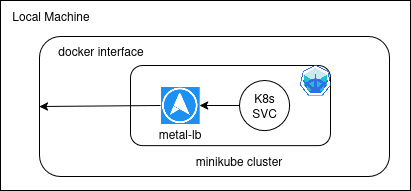
\includegraphics[width=0.8\textwidth]{Design/metal.png}
\end{figure}

From the figure, we can see that MetalLB is intended to be the frontend of our Kubernetes cluster, ingesting data. It's important to note that MetalLB acts as a Layer 4 network load balancer, which allows it to proxy raw UDP packets into our cluster. This solves the problem of ingestion. The traffic will travel to and from the service, to MetalLB, and then to the outside cluster, and vice versa.



\subsubsection{Sequence Flow for MetalLB}
\begin{figure}[H]
\caption{Sequence flow for MetalLB}
\centering
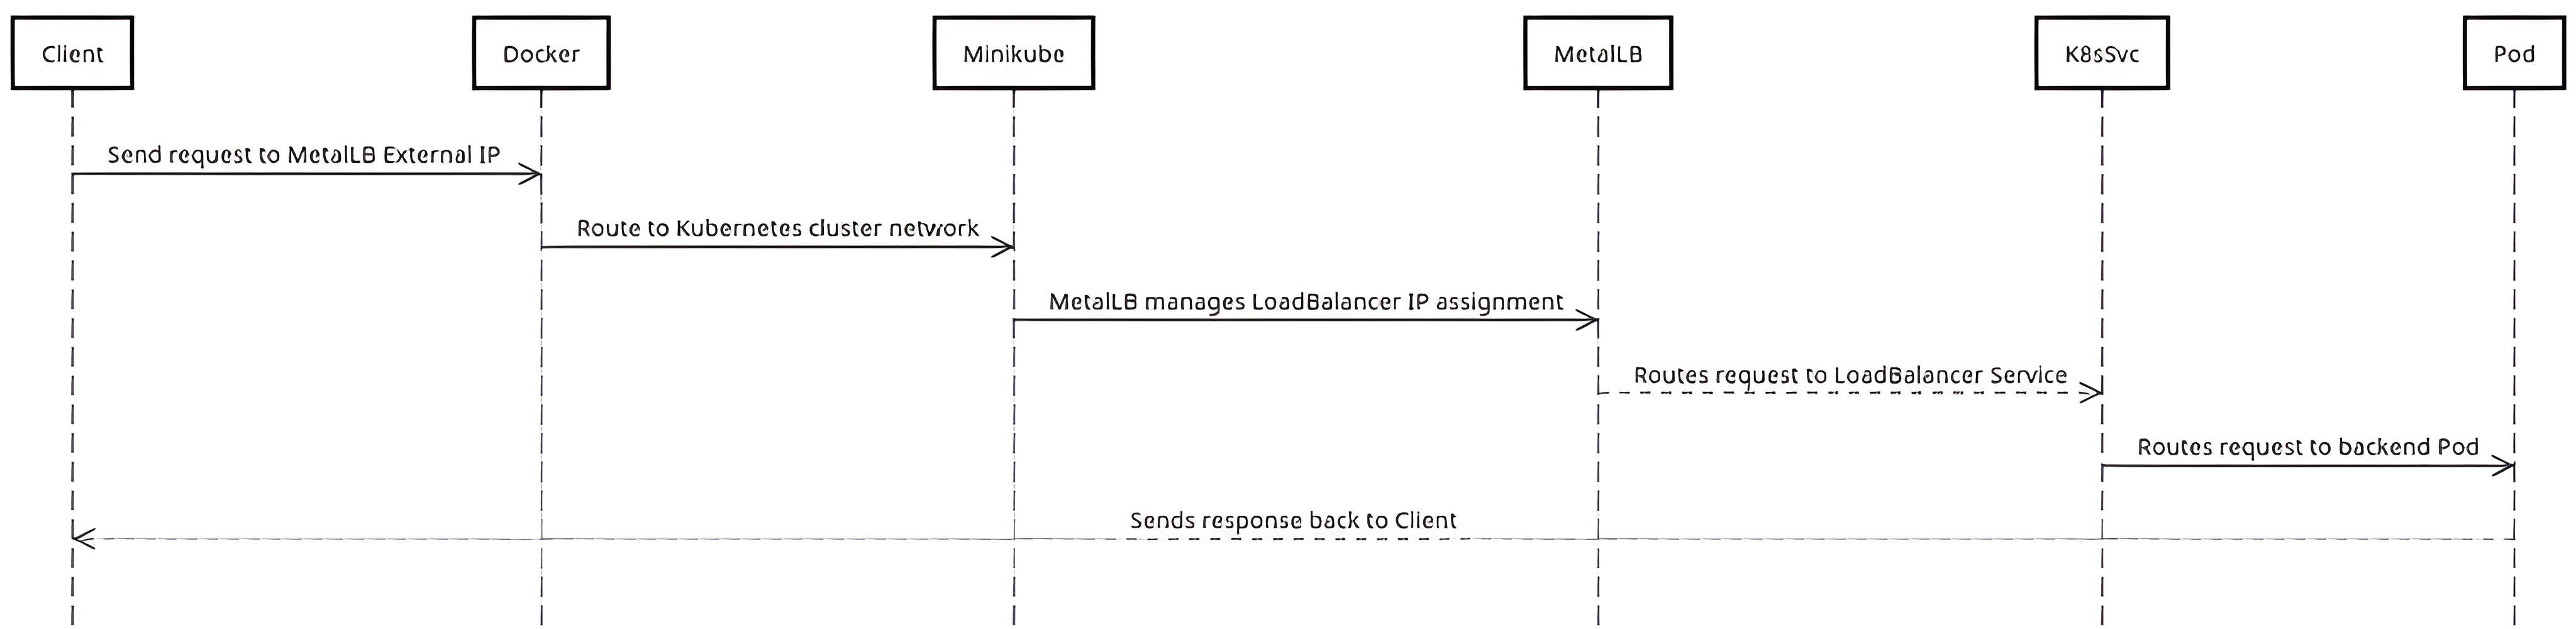
\includegraphics[width=1\textwidth]{Design/metal_sequence.png}
\end{figure}

The client sends a request to the MetalLB IP address. The request is then forwarded through the Docker interface, as MetalLB is deployed on the Minikube cluster, which is running in a Docker container. MetalLB receives the IP address and proceeds to forward the request to the Kubernetes service. This design successfully exposes the Kubernetes service to the outside cluster and allows for the forwarding of raw TCP and UDP packets to our applications.

\section{Design of Backend}

This section presents the design of the routing and processing system for a WebTransport stream-aware routing platform. The design focuses on optimization in configuration, connection management, packet processing, use of metrics, integration of various microservices, and flexibility in command line to facilitate a scalable and resilient streaming design.

\subsection{Configuration-Driven Routing Architecture}



The system adopts a configuration-driven routing approach that allows for dynamic changes and streamlined service management. A central `ServiceConfig` structure defines essential parameters such as host, port, and endpoint for each microservice, such as audio, video, and chat. These configurations are written in a YAML file that is loaded during runtime using a dedicated `ConfigManager` component in Kubernetes. This component enables hot-reloading, so the routing logic can be changed without restarting services. The routing system can therefore be extremely flexible and extensible and easily reconfigured to accommodate emerging needs or varying deployment environments during operation of the system.

The architecture is intended to operate in Kubernetes and utilizes Kubernetes constructs such as ConfigMaps and Secrets to pass routing definitions and TLS credentials to the downstream code. As far as it is concerned, the Router Config is a central configuration file that encapsulates the rules of service routing and protocol behaviors. The router serves as a fast proxy, reading the configuration from this file and redirecting client requests to the correct backend microservices. This decoupled and declarative model leads to routing behavior that is controlled entirely outside of the application's code. This approach aligns with CI/CD principles. The system supports dynamic scaling, safe updates, and operational agility, thereby enabling the router to be deployed in modern cloud-native operations that demand responsiveness and maintainability.


\begin{figure}[h]
\centering
\begin{tikzpicture}[
    box/.style={rectangle, draw, rounded corners, minimum height=2em, minimum width=6em, align=center},
    arrow/.style={-Stealth, thick}
]
    % Nodes
    \node[box] (yaml) at (0,0) {YAML Config};
    \node[box] (manager) at (4.5,0) {ConfigManager};
    \node[box] (service) at (9,0) {ServiceConfig};
    \node[box] (micro) at (13,0) {Microservices};

    % Arrows
    \draw[arrow] (yaml) -- (manager) node[midway, above] {Loads};
    \draw[arrow] (manager) -- (service) node[midway, above] {Parses};
    \draw[arrow] (service) -- (micro) node[midway, above] {Routes};
\end{tikzpicture}
\caption{Configuration-Driven Routing Flow}
\label{fig:config_routing}
\end{figure}

The figure illustrates the flow from a YAML configuration file to the \texttt{ConfigManager}, which parses and stores settings in \texttt{ServiceConfig} structures, enabling routing to microservices. Arrows indicate the sequential process of loading, parsing, and routing configuration data.

\subsection{WebTransport Protocol Handling}

The WebTransport protocol handling system manages QUIC/HTTP3 connections and streams, ensuring reliable communication for real-time streaming. A \texttt{WebTransportRouter} component handles protocol negotiation, stream creation, and HTTP/3 request processing, maintaining connection state. Each QUIC stream is assigned a dedicated buffer to manage packet reassembly and analysis, ensuring efficient handling of incoming data. This design supports high-throughput streaming while maintaining low latency and robust connection management.

\begin{figure}[h]
\centering
\begin{tikzpicture}[
    box/.style={rectangle, draw, rounded corners, minimum height=2em, minimum width=6em, align=center},
    arrow/.style={-Stealth, thick}
]
    % Nodes
    \node[box] (client) at (0,0) {Client};
    \node[box] (router) at (6.5,0) {WebTransportRouter};
    \node[box] (stream) at (13,0) {Stream Buffers};

    % Arrows
    \draw[arrow] (client) -- (router) node[midway, above] {HTTP3 Streams};
    \draw[arrow] (router) -- (stream) node[midway, above] {Assigns};
\end{tikzpicture}
\caption{WebTransport Protocol Handling}
\label{fig:webtransport}
\end{figure}

The figure depicts a client sending data via QUIC/HTTP3 to the \texttt{WebTransportRouter}, which assigns streams to dedicated buffers for processing. Arrows show the flow of data from the client to the router and then to stream buffers.

\subsection{Packet Parsing and Routing}

The packet parsing and routing system is designed to efficiently process incoming packets by extracting headers and forwarding payloads to the correct microservices. A fixed 32-byte header enables fast and reliable parsing, containing fields like \texttt{track\_id}, \texttt{payload\_len}, and \texttt{track\_type}. The payload is extracted based on the \texttt{payload\_len} field and routed to the appropriate microservice using the \texttt{track\_type} and configuration data. This design ensures low-latency processing and accurate routing in a multiplexed streaming environment.

\begin{figure}[h]
\centering
\begin{tikzpicture}[
    box/.style={rectangle, draw, rounded corners, minimum height=1.5em, minimum width=4em, align=center},
    arrow/.style={-Stealth, thick}
]
    % Nodes using absolute positioning
    \node[box] (packet) at (0,0) {Incoming Packet};
    \node[box] (parser) at (6,0) {Packet Parser};
    \node[box] (micro) at (12,0) {Microservices};

    % Arrows
    \draw[arrow] (packet) -- (parser) node[midway, above] {Parses};
    \draw[arrow] (parser) -- (micro) node[midway, above] {Routes};
\end{tikzpicture}
\caption{Packet Parsing and Routing}
\label{fig:packet_parsing}
\end{figure}

The figure shows an incoming packet being processed by the packet parser, which extracts the header and routes the payload to microservices. Arrows indicate the parsing and routing steps.


\subsection{Metrics Logging}
The structure of metrics logging is clearly elaborated in Chapter 6. This part contains the overview of the design 


\begin{figure}[h]
\centering
\begin{tikzpicture}[
    box/.style={rectangle, draw, rounded corners, minimum height=1.5em, minimum width=4em, align=center},
    arrow/.style={-Stealth, thick}
]
    % Nodes
    \node[box] (client) at (0,0) {Client};
    \node[box] (router) at (6,0) {Router};
    \node[box] (logger) at (12,0) {Log to CSV};

    % Arrows
    \draw[arrow] (client) -- (router) node[midway, above] {Sends};
    \draw[arrow] (router) -- (logger) node[midway, above] {Logs};
\end{tikzpicture}
\caption{Client Request Routing and Logging}
\label{fig:client_logging}
\end{figure}


The figure illustrates the system collecting metrics via the \texttt{MetricsLogger}, which logs data to CSV and log files. Arrows represent the flow of metric collection and logging.

\subsection{Microservice Proxying}

The microservice proxying system forwards packets to the appropriate microservices with robust error handling and retry mechanisms. It supports flexible data formats, including binary and JSON, to accommodate different service requirements. Custom headers can be added to packets for extensibility and debugging, enabling traceability and future enhancements. This design ensures reliable communication between the router and microservices, supporting a modular and scalable architecture.



\begin{figure}[h]
\centering
\begin{tikzpicture}[
    box/.style={rectangle, draw, rounded corners, minimum height=1.5em, minimum width=4em, align=center},
    arrow/.style={-Stealth, thick}
]
    \node[box] (router) at (0,0) {Router};
    \node[box] (proxy) at (6,0) {Proxy Layer};
    \node[box] (micro) at (12,0) {Microservices};

    \draw[arrow] (router) -- (proxy) node[midway, above] {Forwards};
    \draw[arrow] (proxy) -- (micro) node[midway, above] {Routes};
\end{tikzpicture}
\caption{Microservice Proxying}
\label{fig:proxying}
\end{figure}

The figure shows the router forwarding packets to a proxy layer, which routes them to microservices with error handling. Arrows depict the forwarding and routing process.



\section{Pulsar Integration Design}

After processing packets such as chat messages, audio streams, or video data, each microservice can optionally publish the output to an Apache Pulsar topic. This mechanism decouples real-time data processing from downstream distribution, analytics, storage, or machine learning. The messages of each particular service are sent to a specifically-named topic, such as chat-topic or video-topic, which guarantees separation of concerns as well as scalability.

This design enables easy integration with real-time data consumers, allows for per-service configuration of Pulsar usage, and allows for flexibility to enable/disable publishing dynamically.



\begin{figure}[h]
\centering
\begin{tikzpicture}[
    box/.style={rectangle, draw, rounded corners, minimum height=2em, minimum width=6em, align=center},
    arrow/.style={-Stealth, thick},
    topic/.style={rectangle, draw, minimum height=2em, minimum width=6em, align=center}
]

% Nodes
\node[box] (micro) at (0,0) {Microservice};
\node[box] (producer) at (4,0) {Pulsar Producer};

% Topic nodes
\node[topic] (chat) at (8,2) {chat-topic};
\node[topic] (video) at (8,0.5) {video-topic};
\node[topic] (audio) at (8,-1) {audio-topic};

% Arrows
\draw[arrow] (micro) -- (producer);
\draw[arrow] (producer) -- (chat);
\draw[arrow] (producer) -- (video);
\draw[arrow] (producer) -- (audio);

\end{tikzpicture}
\caption{Microservice to Pulsar Topics Integration}
\label{fig:microservice_pulsar}
\end{figure}



\section{Complete System Architecture}

The following architecture is a high-level technical architecture diagram which entails the complete proposed solution. The sections above delved deep into each component individually, and this is the final high-level overview of our dissertation.

\begin{figure}[H]
\caption{System Architecture}
\centering
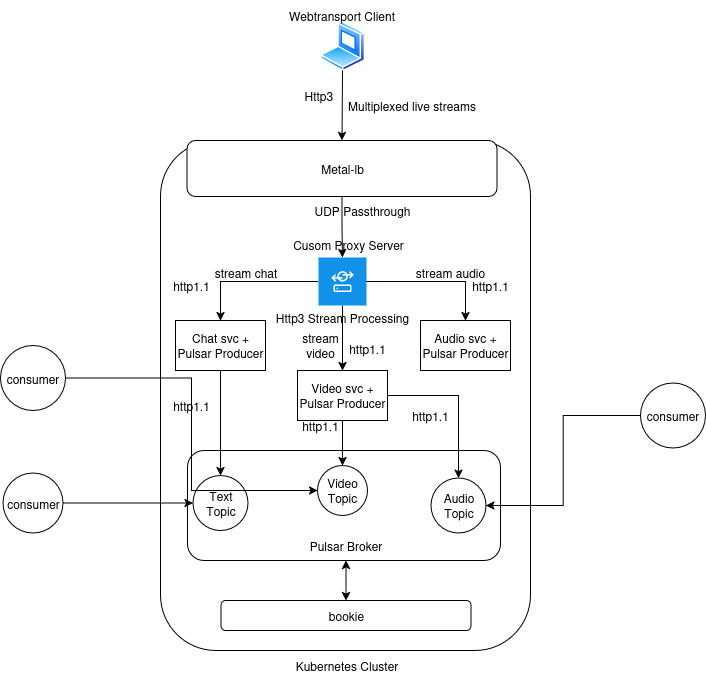
\includegraphics[width=1\textwidth]{Design/Design_Solution.png}
\end{figure}

The proposed architecture system is a real-time streaming system based on a modular structure built to support scaling, low-latency communication, and efficient data processing and distribution within a cloud-native infrastructure. It starts with the ingestion layer where the client sends streams of data with a WebTransport client that connects through HTTP/3, a QUIC-based protocol allowing to establish a single transport connection but with multiplexing multiple data streams in the connection: video, audio, and chat. The load balancer in the Kubernetes cluster is MetalLB, which is exclusively enabled to provide UDP passthrough for the Minikube cluster to facilitate the forwarding of QUIC connections as entire UDP packets to the internal components. The system is centered around a custom proxy server that will terminate the HTTP/3 connection, demultiplex the stream it receives, and forward each individual data stream to the appropriate microservice over HTTP/1.1. This server effectively acts as both a protocol gateway and a routing mechanism.

The application layer is based on different microservices for chat, video, and audio developed which are responsible for handling their own set of data and are independent from each other. These microservices publish the data to Apache Pulsar after processing, acting as a producer in the event streaming system. The Pulsar cluster will have a broker handling the routing and dispatching of messages, different topics that logically segregate each type of data such as Text Topic, Video Topic, Audio Topic, and it will have a persistent storage backend consisting of the Bookie pods of Apache BookKeeper so that persistent data storage and recovery from faults are possible. Finally, on the consumption level, independent consumer applications subscribe to the Pulsar topics and receive data asynchronously. This decouples the data ingestion and downstream processing, enabling use cases of real-time streaming, analytics, or storage with modularity and scalability in the system.
\label{sec:OverviewOfDesign}

\section{Summary}
The proposed system is a real-time streaming architecture that is modular and scalable, designed to support low-latency multimedia communication using WebTransport, Kubernetes, and Apache Pulsar. The architecture breaks the problem space into smaller modules which are developed independently and then combined to form a complete solution. On the client side, WebTransport is used to send data, and WebTransport runs on QUIC to enable data multiplexing across different data streams in a single connection, i.e., audio, video, and chat. The design will prevent Head-of-Line blocking. A typical packet transmitted has a 32-byte header composed of track\_id, payload\_len, and track\_type fields and a variable-length payload. The format is capable of extending; it is useful in routing for a diversity of data types.

Inside the Kubernetes cluster, a single-node Minikube setup is used for simplicity, leveraging the Docker driver to eliminate virtual machine overhead and enable shared networking. MetalLB is used as a bare-metal load balancer that exposes QUIC-based UDP traffic to components of the Kubernetes cluster, enabling external WebTransport clients to connect to internal services. Its routing logic is config-driven, user-managed through YAML-based ConfigMaps, and allows for dynamic updates and reloading of routing configurations without system restarts. The core of this solution is the WebTransportRouter, a custom component that accepts and deals with QUIC/HTTP3 streams by attaching each track with its own explicitly associated buffer of streams. This guarantees that audio, video, and chat information is manipulated on a low-latency basis for redirections. Once the component performs initial parsing, it sends each stream to its respective microservice through HTTP/1.1 via a proxy server that acts as a reliable gateway between the transport and application layers.

At the application layer, separate stateless microservices are responsible for processing specific types of data such as audio, video, or chat. Each microservice publishes the processed data to its corresponding Apache Pulsar topic for instance, chat-topic or video-topic, thereby enabling a decoupled and scalable processing model. Apache Pulsar is used as the main system for handling event streams. It consists of a broker which receives data for a specific topic and stores multiple topics' logical associations, with each topic keeping different types of data separate such as audio, video, or chat. To ensure data is safely stored and can be recovered if something goes wrong, Apache BookKeeper is used in the background through components called Bookies. On the receiving side, different consumer applications connect to Pulsar and subscribe to specific topics to get the data they need. By keeping the parts that send, process, and receive data separate, the system stays flexible, reliable, and easy to scale for real-time streaming or analytics tasks.
